\fontsize{9.5pt}{8.2}\selectfont
\section{Dominio cerrado (Popescu/World)}
\subsection{Introducción}
\begin{frame}
\frametitle{Introducción}
\begin{itemize}
  \item Basado en [Popescu et al. 2003a] y  [Popescu et al. 2003b].
  \item Define \textbf{tratabilidad semántica}
  \item Traduce preguntas semánticamente tratables a \textbf{consultas SQL}
  \item Base de datos relacional de juguete de MySQL, World, con \textbf{información geográfica básica de países, ciudades e idiomas}.
  \item Funcionalidad acotada  $\rightarrow$ soporte solo para el inglés.
\end{itemize}
\end{frame}

\subsection{Modelo teórico}

\begin{frame}[<+->]
  \frametitle{Dominio de problemas / Modelo teórico}
   \begin{block}{Dominio cerrado: acotado y específico}
      \begin{itemize}
          \item Por ejemplo: Restaurants, bancos, vuelos, libros.
          \item Bases de datos relacionales $\rightarrow$ datos estructurados
      \end{itemize}
    \end{block}

  \begin{block}{Modelo teórico}
    \begin{itemize}
          \item Popescu et al. $\rightarrow$ QADB, Precise
          \item QADB: Question answering como interfaz para una base de datos
          \item \textbf{Tratabilidad semántica de una pregunta $q$ en el contexto de una DB $d$}.
          \item Las preguntas no tratables se rechazan, las tratables se traducen a SQL.
          \item Motivación: no se puede fallar activamente (mal interpretar)
    \end{itemize}
  \end{block}
\end{frame}


\begin{frame}
  \frametitle{Ejemplo}
  \begin{block}{Pregunta}<2->
      \textbf{When did Albert Einstein die?}
  \end{block}
  \begin{columns}<3->
      \begin{column}{.5\textwidth}
      \end{column}
      \begin{column}{.1\textwidth}
      \begin{tikzpicture}[>=stealth, rotate border/.style={shape border uses incircle, shape border rotate=270}]
              \node[rotate border=-40, fill=black, minimum height=1.0cm, single arrow, single arrow head extend=.3cm, single arrow head indent=.1cm, inner sep=1.5pt] (arrow) {};
          \end{tikzpicture}
      \end{column}
      \begin{column}{.3\textwidth}
          %Question Answering
      \end{column}
      \begin{column}{.5\textwidth}

      \end{column}
  \end{columns}

  \begin{exampleblock}{Consulta SQL}<3->
\textbf{{\color{purple}SELECT} death\_date \newline
      {\color{purple}FROM} scientists\newline
      {\color{purple}WHERE} name $=$ {\color{green}`Albert Einstein'}
      }
  \end{exampleblock}
  \begin{columns}<4->
      \begin{column}{.5\textwidth}
      \end{column}
      \begin{column}{.1\textwidth}
      \begin{tikzpicture}[>=stealth, rotate border/.style={shape border uses incircle, shape border rotate=270}]
              \node[rotate border=-40, fill=black, minimum height=1.0cm, single arrow, single arrow head extend=.3cm, single arrow head indent=.1cm, inner sep=1.5pt] (arrow) {};
          \end{tikzpicture}
      \end{column}
      \begin{column}{.3\textwidth}
          %Question Answering
      \end{column}
      \begin{column}{.5\textwidth}

      \end{column}
  \end{columns}

  \begin{alertblock}{Respuesta}<4->
      \textbf{April 18th, 1955}
  \end{alertblock}

\end{frame}


\begin{frame}[<+->]
  \frametitle{Tratabilidad semántica / motivación}
      \begin{itemize}
          \item La complejidad de las preguntas en lenguaje natural es arbitrariamente grande.
          \item Distinguir un subconjunto 1) \textit{tratable} y 2) \textit{abarcativo}
          \begin{itemize}
            \item La {\color{blue}\textbf{tratabilidad semántica}} define ese conjunto
          \end{itemize}
          \item Rechazar y pedir reformulación de las no tratables
          \begin{itemize}
            \item Es mejor no dar respuesta a dar una mala. 
            \item Conservar la confianza en el sistema.
          \end{itemize}
      \end{itemize}
\end{frame}

\begin{frame}[<+->]
  \frametitle{Tratabilidad semántica / intuición}
    \begin{block}{Tratabilidad semántica en el contexto de una DB}
      \begin{itemize}
          \item Una {\color{green}Q-word} (Qué, quién, cuándo, dónde, etc.)
          \item Pares de {\color{blue}atributos} y {\color{blue}valores}
          \item {\color{purple}Valores} sueltos
          \item Términos no significativos y {\color{orange}menciones a relaciones}
          \item Por ejemplo:
            \begin{itemize}
              \item ¿{\color{green}Qué} {\color{orange}bancos} de la {\color{red}empresa Credicoop} están localizados en el {\color{blue}barrio} de {\color{blue}Coghlan}?
              \item ¿{\color{green}Quién} era el {\color{red}presidente} de {\color{red}México} en {\color{purple}1993}?
            \end{itemize}
      \end{itemize}
    \end{block}
\end{frame}

\fontsize{9.5pt}{7.2}\selectfont
\begin{frame}[<+->]
  \frametitle{Elemento, qword, compatibilidad}
   \begin{itemize}
      \item \textbf{Elementos} de una DB: Relaciones, Atributos y Valores
      \item \textbf{Qwords} - pronombres interrogativos
      \begin{itemize}
          \item \{What, where, which, when, who\}
          \item \{Qué, dónde, cuál, cuándo, quién\}
      \end{itemize}
      \item \textbf{Compatibilidad}
      \begin{itemize}
          \item Valor $\rightarrow$ atributo (Macri $\rightarrow$ HeadOfState)
          \item Atributo  $\rightarrow$  relación (HeadOfState $\rightarrow$ Country)
          \item Valor $\rightarrow$ relaciones de sus atributos (Macri $\rightarrow$ Country)
          \item {\color{blue}Q-words $\rightarrow$ atributos}
          \begin{itemize}
            \item Definición a mano especifica por DB
            \item Who $\rightarrow$ HeadOfState
            \item When $\rightarrow$ IndependenceYear 
          \end{itemize}
      \end{itemize}
    \end{itemize}
\end{frame}


\begin{frame}[<+->]
  \frametitle{Token, marcador sintáctico}
   \begin{itemize}
          \item \textbf{Token}: un conjunto de (lemas de) palabras que corresponden a un elemento de la base de datos.
      \begin{itemize}
            \item Por ejemplo, \{experiencia, requerir\} y \{experiencia, necesario\} son dos tokens para ``Experiencia Requerida''
            \item El {\color{red}\textbf{lexicón}} genera todos los tokens válidos a partir de los elementos de la DB usando Wordnet
      \end{itemize}
      \item \textbf{Marcador sintáctico} (stopword):
      \begin{itemize}
        \item Palabras que no aportan y se tiran (v.gr: y, el, la, etc.)
        \item Definidas a mano. Problemático.
      \end{itemize}
    \end{itemize}
\end{frame}


\fontsize{9.5pt}{7.2}\selectfont
\begin{frame}[<+->]
  \frametitle{Lexicón: definición del espacio semántico a partir de la DB}
  Correspondencia entre tokens y elementos
  \begin{itemize}
    \item Separa cada elemento en palabras individuales:
    \begin{itemize}\fontsize{9.5pt}{7.2}\selectfont
      \item “ExperienciaRequerida” $\rightarrow$ \{Experiencia, Requerida\}
    \end{itemize}
    \item Sinónimos para cada palabra usando Wordnet:
    \begin{itemize}\fontsize{9.5pt}{7.2}\selectfont
      \item experiencia $\rightarrow$ \{experiencia, conocimiento, habilidad,...\}
      \item requerida $\rightarrow$ \{requerida, necesaria, indispensable,...\}
    \end{itemize}
    \item Lematizar:
      \begin{itemize}\fontsize{9.5pt}{7.2}\selectfont
        \item experiencia $\rightarrow$ \{experiencia, conocimiento, habilidad,...\}
        \item requerida $\rightarrow$ \{requerir, necesario, indispensable,...\}
    \end{itemize}
    \item Combinar:
    \begin{itemize}\fontsize{9.5pt}{7.2}\selectfont
        \item tokens = \{(experiencia, requerir), (conocimiento, requerir), (habilidad, requerir),(experiencia, necesario), (conocimiento, necesario), (habilidad, necesario),(experiencia, indispensable), (conocimiento, indispensable), (habilidad, indispensable)\}
    \end{itemize}
    \item Un token \textit{\textbf{corresponde}} a un elemento
    \begin{itemize}\fontsize{9.5pt}{7.2}\selectfont
    \item (habilidad, indispensable) corresponde a ExperienciaRequerida
    \end{itemize}
  \end{itemize}
\end{frame}




\begin{frame}[<+->]
\frametitle{Tokenización completa, asociación sintáctica}

  \begin{itemize}
    \item \textbf{Tokenización completa de una pregunta \textit{q}}:  cualquier conjunto de tokens en los que cada término que no es un marcador sintáctico de $q$ aparece en exactamente un token del conjunto.
    \begin{itemize}
      \item Una partición de tokens de la pregunta $q$
      \item Para ser tratable, $q$ tiene que tener \textit{solo} stopwords y tokens del lexicón.
    \end{itemize} 
    \item \textbf{Asociación sintáctica}: dos tokens están sintácticamente asociados en $q$ si cumplen ciertas restricciones sintácticas.
    \begin{itemize}
      \item Modelado con una función $attachment($ t1, t2, q $) \rightarrow booleano$
    \end{itemize} 
   \end{itemize}
\end{frame}

\fontsize{9.5pt}{7.2}\selectfont
\begin{frame}[<+->]
\frametitle{Traducción válida}
 Una \textbf{traducción válida} es un mapeo de una tokenización completa de $q$ en elementos de $E$ que cumple 3 condiciones:
\begin{enumerate}
  \item Cada token se corresponde con un único elemento de $E$.
  \item Cada token de atributo se relaciona con un único token de valor, cumpliendo que:
  \begin{itemize}
    \fontsize{9.5pt}{7.2}\selectfont
    \item el atributo de la base de datos que corresponde al token de atributo y el valor de la base de datos que corresponde al token de valor son compatibles
    \item ambos tokens están sintácticamente asociados \footnotemark 
   \end{itemize}
\end{enumerate}
\footnotetext[1]{\tiny{Falta una condición sobre tokens de relación que no usamos en la tesis}}
\end{frame}

\fontsize{10pt}{11.2}\selectfont
\begin{frame}[<+->]
\frametitle{Tratabilidad semántica - formalización}
Una pregunta es \textbf{semánticamente tratable} si:
\begin{itemize}
  \item Tiene una y solo una q-word 
  \item Tiene al menos una traducción válida
\end{itemize}

\bigskip
\bigskip

Una traducción válida de $q$ se traduce trivialmente a una query SQL:
\bigskip
\centering
\begin{tabular}{ r | l }
SELECT &  Elementos apareados con qwords \\
WHERE & Pares de atributos y valores apareados\\
FROM & Todas las relaciones mencionadas \\
\end{tabular}
\end{frame}

\fontsize{11pt}{7.2}\selectfont
\begin{frame}
\frametitle{Ejemplo}
\begin{figure}
  \centering
    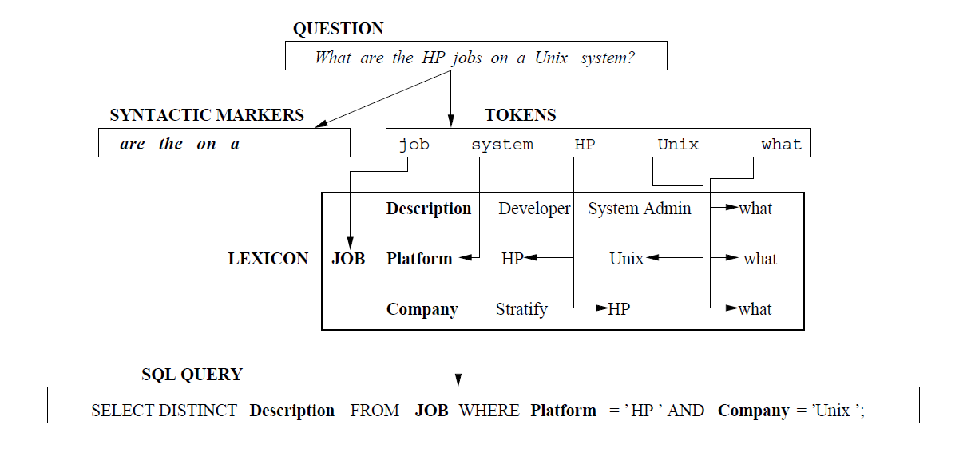
\includegraphics[scale=.7]{graficos/popescu-example}
  \caption{La traducción de la pregunta ``What are the HP jobs on a Unix system?'' a una consulta SQL}
  \label{fig:popescu-example}
\end{figure}
\end{frame}


\fontsize{9.5pt}{7.2}\selectfont
\begin{frame}
\frametitle{Módulos de Precise}
   \begin{block}{Lexicon}<1->
      \begin{itemize}
          \item Sinónimos lematizados de todas las relaciones, atributos y valores
          \begin{itemize}
            \item Wordnet
          \end{itemize}
          \item Determina qué términos son comprensibles de una pregunta
          \item Las preguntas tratables tienen solamente marcadores sintácticos + palabras del lexicon.
        \end{itemize}
    \end{block}
    \begin{block}{Tokenizer}<1->
      \begin{itemize}
          \item Rompe la pregunta y consulta al lexicón
          \item Genera tokenizaciones completas que alimentan al Matcher
          \item Propone mapeos entre palabras y elementos de la DB (tokenizaciones completas)
      \end{itemize}
    \end{block}
  
\end{frame}

\begin{frame}
\frametitle{Módulos de Precise (2)}

    \begin{block}{Matcher}<1->
      \begin{itemize}
          \item La pieza clave.
          \item Relaciona cada valor con un único atributo, implícito o explícito usando un algoritmo de max flow.
          \item Selecciona mapeos válidos (traducciones válidas)
      \end{itemize}
    \end{block}
    \begin{block}{Otros}<1->
      \begin{itemize}
        \item Parser plug-in: computa la función de asociación sintáctica, basándose en el parse tree de Charniak.
        \item Query generator: dado el conjunto de elementos de la base de datos traducido de la pregunta, genera una query SQL.
        \item Equivalence Checker: verifica si diferentes queries son la misma formulada de diferentes maneras.
      \end{itemize}
    \end{block}
\end{frame}


\begin{frame}

\frametitle{Ejemplo}

\begin{figure}
  \centering
    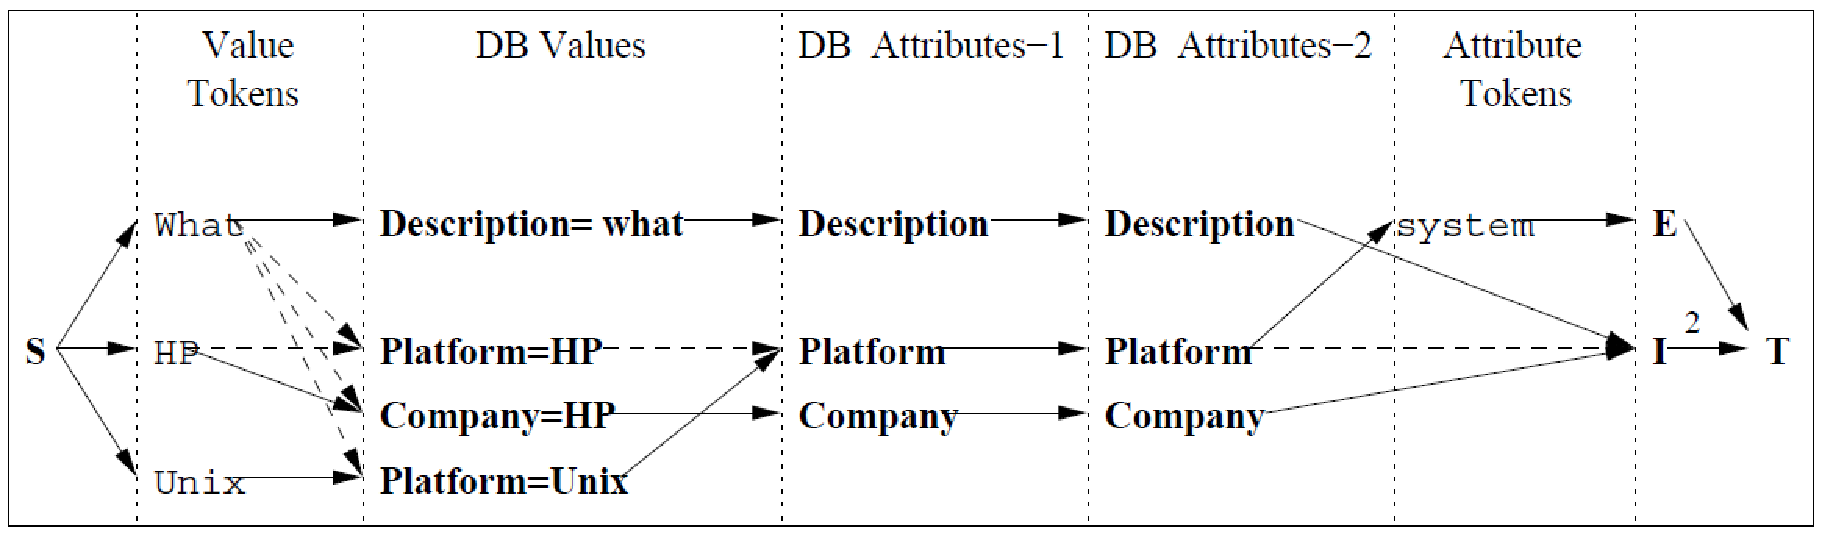
\includegraphics[scale=0.3]{graficos/popescu-example-2}
  \caption{El grafo de atributos y valores del Matcher para la pregunta ``What are the HP jobs on a Unix system?''}
  \label{fig:popescu-example-2}
\end{figure}
\end{frame}

\subsection{Implementación}

\subsubsection*{Base de datos}
\begin{frame}
\frametitle{Base de datos: World (Country, City y CountryLanguage)}
\begin{figure}
    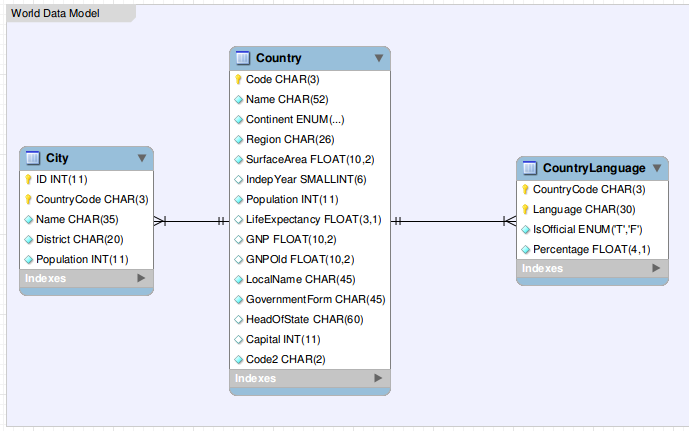
\includegraphics[width=9.823cm,height=6.004cm]{graficos/fuentes/world-db.png}
\end{figure}
\end{frame}


\subsubsection*{Implementación}


\fontsize{9.5pt}{7.2}\selectfont
\begin{frame}[<+->]
\frametitle{Implementación: Lexicón, Tokenize}
  Seguimos las indicaciones dadas sobre Precise

  \begin{block}{Lexicón: genera el espacio semántico.}
    \begin{itemize}
      \item \fontsize{7.5pt}{7.2}\selectfont Elemento DB (Relación, Atributo, Valor) $\rightarrow$ Wordnet $\rightarrow$ Lexicón
      \item \fontsize{7.5pt}{7.2}\selectfont Notas: TokenAugmenter. Polisemia. Problemas.
    \end{itemize}
  \end{block}
  \begin{block}{Tokenizer: particiona la pregunta en tokens del lexicón}
      \begin{enumerate}
        \item \fontsize{7.5pt}{7.2}\selectfont Separar la pregunta en palabras, eliminar puntuaciones y pasar a lower case
        \item \fontsize{7.5pt}{7.2}\selectfont Lematizar las palabras
        \item \fontsize{7.5pt}{7.2}\selectfont Eliminar marcadores sintácticos
        \item \fontsize{7.5pt}{7.2}\selectfont Para cada lema, obtener todos los tokens que lo contienen del Lexicon
        \item \fontsize{7.5pt}{7.2}\selectfont Para cada token potencial, verificar que todos sus lemas estén presentes en la pregunta original.
        \item \fontsize{7.5pt}{7.2}\selectfont Generar el conjunto de partes de todos los tokens filtrados
        \item \fontsize{7.5pt}{7.2}\selectfont Para cada uno de estos subconjuntos, verificar 1) que sus tokens cubran completamente los lemas significativos de la pregunta original y 2) que no haya lemas repetidos entre los tokens.
        \end{enumerate}
  \end{block}
\end{frame}

\begin{frame}[<+->]
\frametitle{Implementación: Matcher}
  
  \begin{itemize}
    \item Input = tokenizaciones completas generadas por el Tokenizer,
    \item Construye el grafo atributo valor
    \item Algoritmo de max flow.
    \item Las aristas implicadas en el flujo máximo posible asocian 
    \begin{enumerate}
      \item los tokens de valor y de atributo y los correspondientes elementos (valores y atributos, respectivamente) de la DB y 
      \item pares de valores y atributos entre sí.
    \end{enumerate}
    \item Más de una solución posible: todos los flujos máximos son en principio traducciones válidas.
\end{itemize}

\end{frame}

        % \begin{frame}
        % \frametitle{Implementación - Condiciones semánticas y sintácticas de la traducción}

        % Finalmente, verificamos cuales de las soluciones con máximo flujo cumplen las condiciones requeridas para ser una traducción válida según enu

        % \begin{enumerate}
        % \item Todos  los tokens de la tokenización tienen un único elemento de la base de datos asociado y no hay elementos de la base de datos repetidos. (Mapping.meetsConditionOne())
        % \item Cada token de atributo se relaciona con un único token de valor respetando que: (Mapping.meetsConditionTwo())
        % \begin{enumerate}
        % \item el atributo relacionado con el token de atributo y el valor relacionado con el token de valor son compatibles (esta condición está garantizada por el max-flow mismo)
        % \item ambos tokens están sintácticamente asociados
        % \end{enumerate}
        % \item Cada token de relación está relacionado a un token de atributo o bien a un token de valor, cumpliendo las siguientes condiciones:
        % \begin{enumerate}
        % \item la relación de la base de datos que corresponde al token de relación y el elemento de la base de datos que corresponde al token de atributo o token de valor son compatibles
        % \item ambos tokens (token de relación - token de atributo o bien token de relación - token de valor) están sintácticamente asociados
        % \end{enumerate}
        % \item La pregunta tiene una qword
        % \end{enumerate}
        % \end{frame}


\begin{frame}
\frametitle{Implementación: Charniak parser - chequeo sintáctico}
\begin{itemize}
\item No especificado por los autores
\item Escribimos reglas propias que vinculan hoja sustantivo, adjetivo o adverbio y qwords
\end{itemize}

\end{frame}


\begin{frame}
\frametitle{Charniak parse tree}
\Tree [.S1 [.WHNP [.WP What ] ] [.SQ [.VP [.AUX are ] [.{\color{red}NP} [.DT the ] [.{\color{red}NNP} {\color{red}HP} ] [.{\color{red}NNS} {\color{red}jobs} ] ] [.PP [.IN on ] [.{\color{red}NP} [.DT a ] [.{\color{red}NNP} {\color{red}Unix} ] [.{\color{red}NN} {\color{red}system} ] ] ] ] ] [.. ? ] ] \\
{\color{red}Regla 1 - Sustantivos \dq{hermanos}}

\end{frame}

\begin{frame}
\frametitle{Charniak parse tree}
\Tree [.{\color{blue}S1} [.{\color{blue}WHNP} [.{\color{blue}WP} {\color{blue}What} ] ] [.{\color{blue}SQ} [.{\color{blue}VP} [.AUX are ] [.{\color{blue}NP} [.DT the ] [.{\color{blue}NNP} {\color{blue}HP} ] [.{\color{blue}NNS} {\color{blue}jobs} ] ] [.PP [.IN on ] [.NP [.DT a ] [.NNP Unix ] [.NN system ] ] ] ] ] [.. ? ] ] \\
{\color{blue}Regla 2: qwords a sustantivos}

\end{frame}

\begin{frame}
\frametitle{Charniak parse tree}
\Tree [.S1 [.WHNP [.WP What ] ] [.SQ [.{\color{purple}VP} [.AUX are ] [.{\color{purple}NP} [.DT the ] [.{\color{purple}NNP} {\color{purple}HP} ] [.NNS jobs ] ] [.{\color{purple}PP} [.IN on ] [.{\color{purple}NP} [.DT a ] [.{\color{purple}NNP} {\color{purple}Unix} ] [.{\color{purple}NN} {\color{purple}system} ] ] ] ] ] [.. ? ] ] \\
{\color{purple}Regla 3: sintagma nominal a sintagma preposicional}

\end{frame}

\begin{frame}
\frametitle{Charniak parse tree}
\Tree [.S1 [.WHNP [.WP What ] ] [.SQ [.{\color{purple}VP} [.AUX are ] [.{\color{purple}NP} [.DT the ] [.NNP HP ] [.{\color{purple}NNS} {\color{purple}jobs} ] ] [.{\color{purple}PP} [.IN on ] [.{\color{purple}NP} [.DT a ] [.{\color{purple}NNP} {\color{purple}Unix} ] [.{\color{purple}NN} {\color{purple}system} ] ] ] ] ] [.. ? ] ] \\
{\color{purple}Regla 3: sintagma nominal a sintagma preposicional (otra)}

\end{frame}


              % \begin{frame}
              % \frametitle{Algunas notas}
              %  No usar charniak. Mejora la performance. Empeora filtro. Mas desambiguaciones mas tontas.

              % Finalmente, todos los resultados de max-flow que cumplen con las condiciones de 1 a  4 son traducciones válidas, que pasan al MappingFilter, que realiza ciertos filtrados que describiremos, de nuevo, en un título aparte.

              % Resultado e Mappings (una estructura que contiene 1) una tokenización completa de la pregunta original y 2) un mapeo válido entre cada token de la misma en un elemento de la base de datos). 
              % Cada mapeo es una traducción válida de la pregunta. Si existe solo uno, entonces este mapeo se traducirá en una query que generará el resultado. Si no, corresponde al MappingFilter realizar filtrados inteligentes de las múltiples soluciones y, en caso de que continuen existiendo múltiples soluciones, entonces se consultará al usuario qué quiso preguntar. Por otro lado, si no fue posible generar ninguna traducción válida, se retornará al usuario sin respuesta, pidiéndole que vuelva a escribir su pregunta de otro modo.


              % \end{frame}


              % \begin{frame}
              % \frametitle{Filtros, Generación de queries}

              % \textbf{MappingFilter}
              % \begin{itemize}
              % \item Elimina repetidas (según su query SQL).
              % \item Regla 1 - ``semi duplicados'': atributos similares de la DB\footnotemark 
              % \item Regla 2 y 3 - Fundamento. si una traducción válida tiene su qword asociado a un atributo \textit{implícito}, también estará asociado con todos los atributos que pueda estarlo (ver tabla table:atributos-qwords para las compatibilidades definidas).\footnotemark 
              % \item Regla 2 - Preferir, entre los atributos implícitos, aquellos cuya relación está mencionada en la pregunta (si hubiera alguna). 
              % \item Regla 3 - Una vez especificada la relación, priorizar el atributo implicito preferido en negrita en la tabla table:atributos-qwords. 
              % \item Si después de MappingFilter hay más de una traducción, vuelve al usuario a desambiguar
              % \end{itemize}
              % \textbf{QueryGenerator}

              % \centering
              % \begin{tabular}{ r | l }
              % SELECT &  Elementos apareados con qwords \\
              % WHERE & Pares de atributos y valores generados por el Matcher\\
              % FROM & Todas las relaciones mencionadas \\
              % \end{tabular}



              % \footnotetext[1]{ en concreto, una query que consulta por Country.Name Country.LocalName}
              % \footnotetext[2]{Esto implica que, por ejemplo, para cualquier pregunta cuya qword sea 'what' y no tenga su atributo asociado explícito, habrá 16 diferentes traducciones válidas.}

              % \end{frame}

\subsubsection*{Ejemplos}
\begin{frame}
\frametitle{Ejemplos}
  \begin{enumerate}
    \item Who is the head of state of Zimbabwe?
    \bigskip
    \item What caribbean countries are also considered north american?
  \end{enumerate}
\end{frame}

\begin{frame}[t]
\frametitle{Ejemplo 1: ``Who is the head of state of Zimbabwe?''}
Ejemplo 1:\newline
  \Large{``Who is the head of state of Zimbabwe?''}
\end{frame}

\begin{frame}[t]
\frametitle{Ejemplo 1: Tokenizer}
1. Separar en palabras, eliminar puntuaciones y pasar a lower case:\newline
  \Large{``{\color{blue}w}ho is the head of state of {\color{blue}z}imbabwe{\color{red}\st{?}}''}
\end{frame}


\begin{frame}[t]
\frametitle{Ejemplo 1: Tokenizer}
1. Separar en palabras, eliminar puntuaciones y pasar a lower case:\newline
  \Large{\{{\color{blue}w}ho, is, the, head, of, state, of, {\color{blue}z}imbabwe\}}
\end{frame}
\begin{frame}[t]
\frametitle{Ejemplo 1: Tokenizer}
2. Lematizar las palabras, eliminar marcadores sintácticos:\newline
  \Large{\{who, {\color{red}\st{is}}, {\color{red}\st{the}}, head, {\color{red}\st{of}}, state, {\color{red}\st{of}}, zimbabwe\}}
\end{frame}

\begin{frame}[t]
\frametitle{Ejemplo 1: Tokenizer}
2. Lematizar las palabras, eliminar marcadores sintácticos:\newline
  \Large{\{who, head, state, zimbabwe\}}
\end{frame}

\begin{frame}[t]
\frametitle{Ejemplo 1: Tokenizer - tokens para who}
3. Obtener tokens para cada lema \newline
    \Large{$getTokens(who)\ \rightarrow \{$'who'$\}$}
\end{frame}

\begin{frame}[t]
\frametitle{Ejemplo 1: Tokenizer - tokens para head}
3. Obtener tokens para cada lema \newline
    \Large{$
    getTokens(head)\ \rightarrow \{$ 'head country', 'head teacher body politic', 'head body politic', 'head teacher land', 'read / write head dos', 'heading provincial', 'heading state', 'heading commonwealth', 'read / write head body politic', 'head word land', 'head state of matter', 'read / write head provincial', 'read / write head state department', 'head province',  'heading res publica', 'read / write head nation', (51 más)...$\}$}
\end{frame}

\begin{frame}[t]
\frametitle{Ejemplo 1: Tokenizer - tokens para state}
3. Obtener tokens para cada lema \newline
  \Large{ $getTokens(state)\ \rightarrow  \{$'heart eastern united states', 'centre eastern united states', 'central eastern united states', 'centrical eastern united states', 'midsection eastern united states', 'midriff eastern united states', 'centric eastern united states', 'center eastern united states', 'north western united states', (702 más)...$\}$}
\end{frame}

\begin{frame}[t]
\frametitle{Ejemplo 1: Tokenizer - tokens para Zimbabwe}
3. Obtener tokens para cada lema \newline
  \Large{$getTokens(zimbabwe)\ \rightarrow \{$'zimbabwe', 'republic of zimbabwe', 'capital of zimbabwe'$\}$}

\end{frame}

\begin{frame}[t]
\frametitle{Ejemplo 1: Tokenizer - intersección}
4. Filtrar solo tokens cuyos lemas estén en la pregunta\newline
  \Large{$getTokens(zimbabwe)\ \rightarrow \{$'zimbabwe', {\color{red}\st{'republic of zimbabwe'}}, {\color{red}\st{'capital of zimbabwe'}}$\}$ }
\end{frame}


\begin{frame}[t]
\frametitle{Ejemplo 1: Tokenizer - intersección}
4. Filtrar solo tokens cuyos lemas estén en la pregunta\newline
  \Large{$getTokens(zimbabwe)\ \rightarrow \{$'zimbabwe'$\}$}
\end{frame}


\begin{frame}[t]
\frametitle{Ejemplo 1: Tokenizer - intersección}
4. Filtrar solo tokens cuyos lemas estén en la pregunta\newline
  \Large{
    $getTokens(zimbabwe) \rightarrow \{$'zimbabwe'$\}$\newline
    $getTokens(who)\ \rightarrow \{$'who'$\}$\newline
    $getTokens(head) \rightarrow \{$'head state','heading state'$\}$\newline
    $getTokens(state) \rightarrow  \{$'state','head state','heading state'$\}$
}
\end{frame}

\begin{frame}[t]
\frametitle{Ejemplo 1: ``Who is the head of state of Zimbabwe?''}
 5. Generar el conjunto de partes de todos los tokens.\newline
  \Large{
      $\emptyset$,\newline
      \{'zimbabwe', 'state'\},\newline
      \{'zimbabwe', '{\color{red}state}', 'head {\color{red}state}', 'who'\},\newline
      \{'head state', 'zimbabwe', 'who'\},\newline
      \{'{\color{red}heading state}', 'zimbabwe', '{\color{red}head state}', 'who'\},\newline
      ...
  }\newline

  \normalsize{Para cada uno de estas \textit{tokenizaciones}, verificar:
  \begin{itemize}
    \item Que sus palabras cubran la pregunta original.
    \item Que no haya palabras repetidas entre los tokens.
  \end{itemize}
  }
\end{frame}

\begin{frame}
\frametitle{Ejemplo 1: Tokenizaciones completas}

\begin{center}

$q = \text{``Who is the head of state of Zimbabwe?''}$
\end{center}
 \begin{equation*}
    CompleteTokenizations(q) = \begin{cases}
               \text{who, head state, zimbabwe} \\
               \\
               \\
               \text{who, heading state, zimbabwe} \\
           \end{cases}
\end{equation*}

\end{frame}

\begin{frame}[t]
\frametitle{Ejemplo 1: Lexicón - Tokens $\rightarrow$ Elementos}
Obtener elementos de la DB para cada token\newline
  \Large{
    $zimbabwe \rightarrow Zimbabwe$ (Valor de Country.Name)
    }
\end{frame}

\begin{frame}[t]
\frametitle{Ejemplo 1: Lexicón - Tokens $\rightarrow$ Elementos}
Obtener elementos de la DB para cada token\newline
  \Large{
    $\text{head state} \rightarrow HeadOfState$ (Atributo de Country)
    }
\end{frame}

\begin{frame}[t]
\frametitle{Ejemplo 1: Lexicón - Tokens $\rightarrow$ Elementos}
Obtener elementos de la DB para cada token\newline
  \Large{
    $\text{heading state} \rightarrow HeadOfState$ (Atributo de Country)
    }
\end{frame}

\begin{frame}[t]
\frametitle{Ejemplo 1: Lexicón - Tokens $\rightarrow$ Elementos}
Obtener elementos de la DB para cada token\newline
  \Large{
    $who \rightarrow Who$ (Qword compatible con HeadOfState)
    }
\end{frame}

\begin{frame}
\frametitle{Ejemplo 1: Matcher - Grafo de atributos y valores}
\begin{figure}
  \centering
    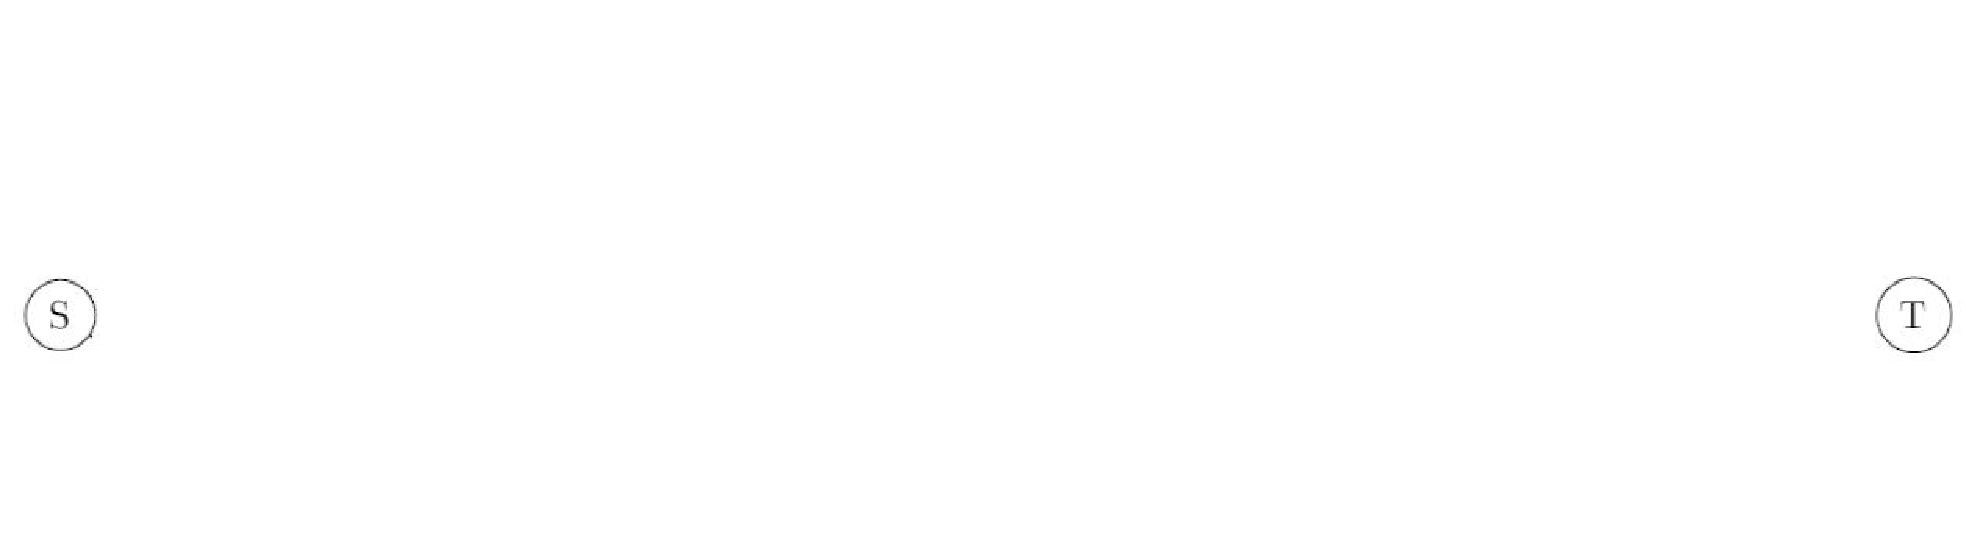
\includegraphics[scale=.33]{graficos/presentacion/ejemplo-grafo-matcher-1-2}
\end{figure}
\end{frame}

\begin{frame}
\frametitle{Ejemplo 1: Matcher - Grafo de atributos y valores}
\begin{figure}
  \centering
    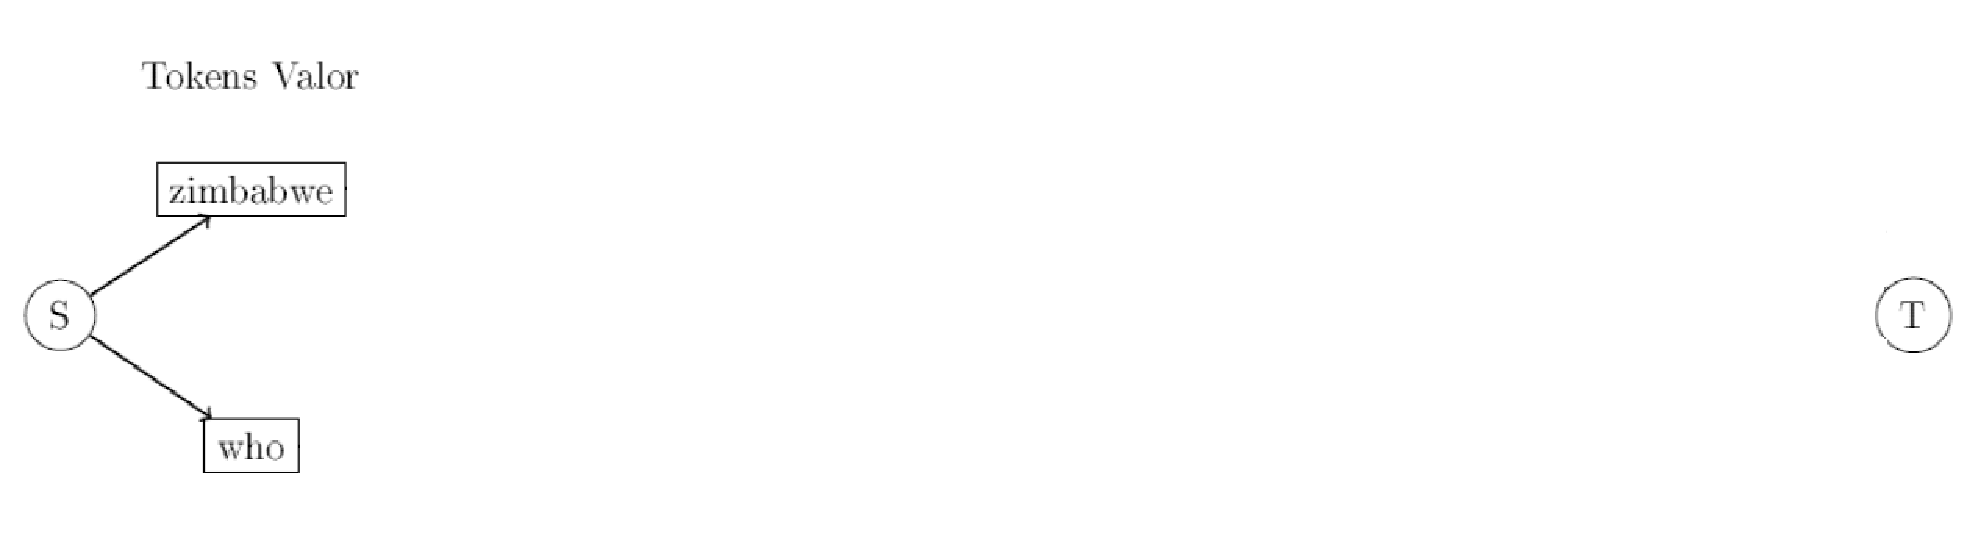
\includegraphics[scale=.33]{graficos/presentacion/ejemplo-grafo-matcher-1-3}
\end{figure}
\end{frame}

\begin{frame}
\frametitle{Ejemplo 1: Matcher - Grafo de atributos y valores}
\begin{figure}
  \centering
    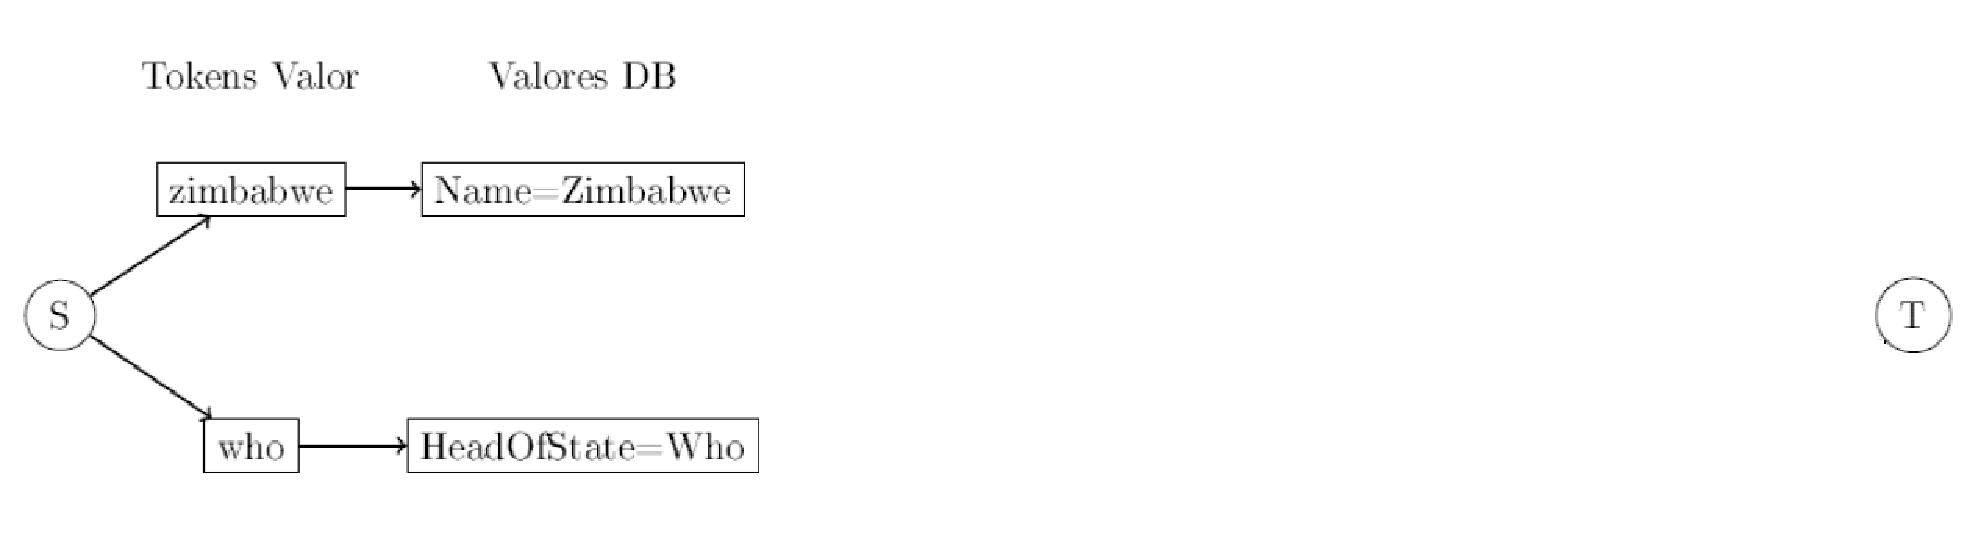
\includegraphics[scale=.33]{graficos/presentacion/ejemplo-grafo-matcher-1-4}
\end{figure}
\end{frame}

\begin{frame}
\frametitle{Ejemplo 1: Matcher - Grafo de atributos y valores}
\begin{figure}
  \centering
    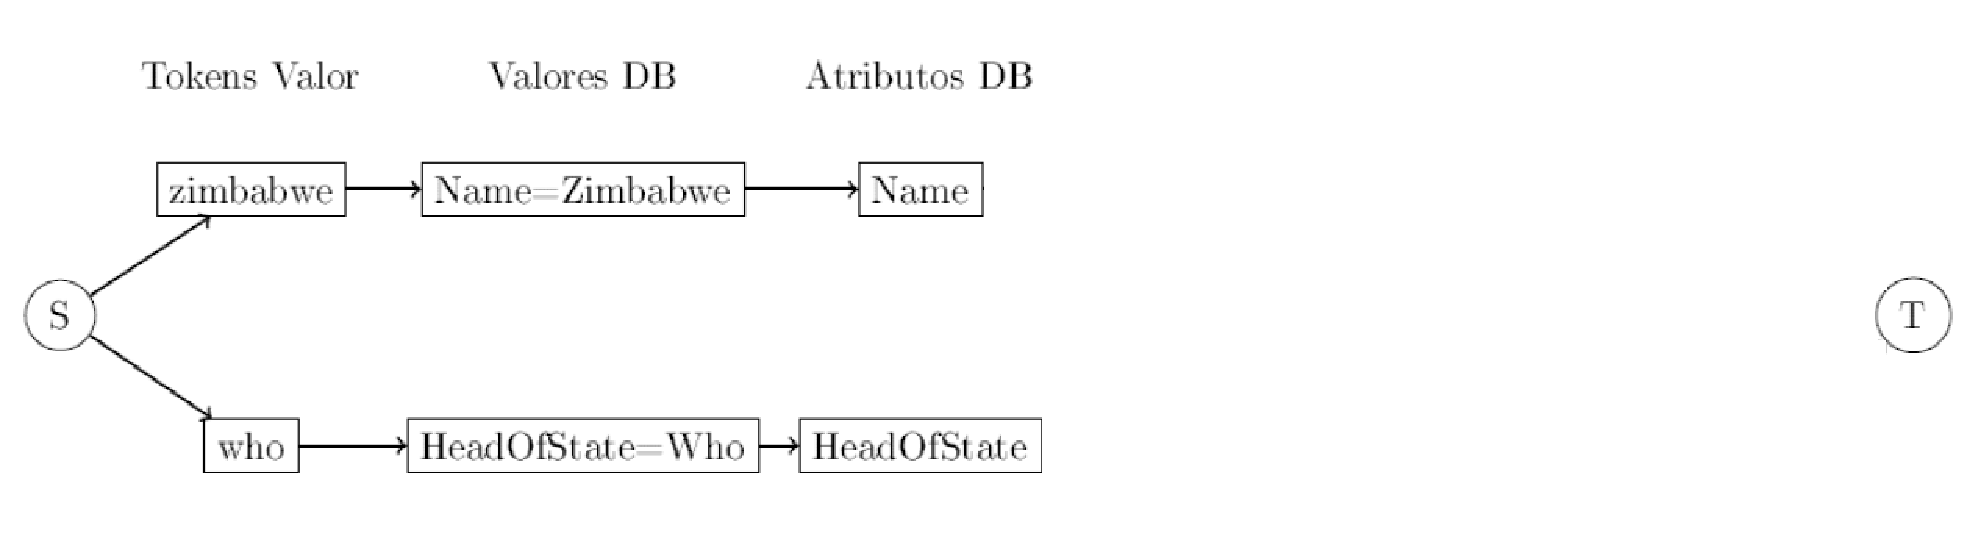
\includegraphics[scale=.33]{graficos/presentacion/ejemplo-grafo-matcher-1-5}
\end{figure}
\end{frame}

\begin{frame}
\frametitle{Ejemplo 1: Matcher - Grafo de atributos y valores}
\begin{figure}
  \centering
    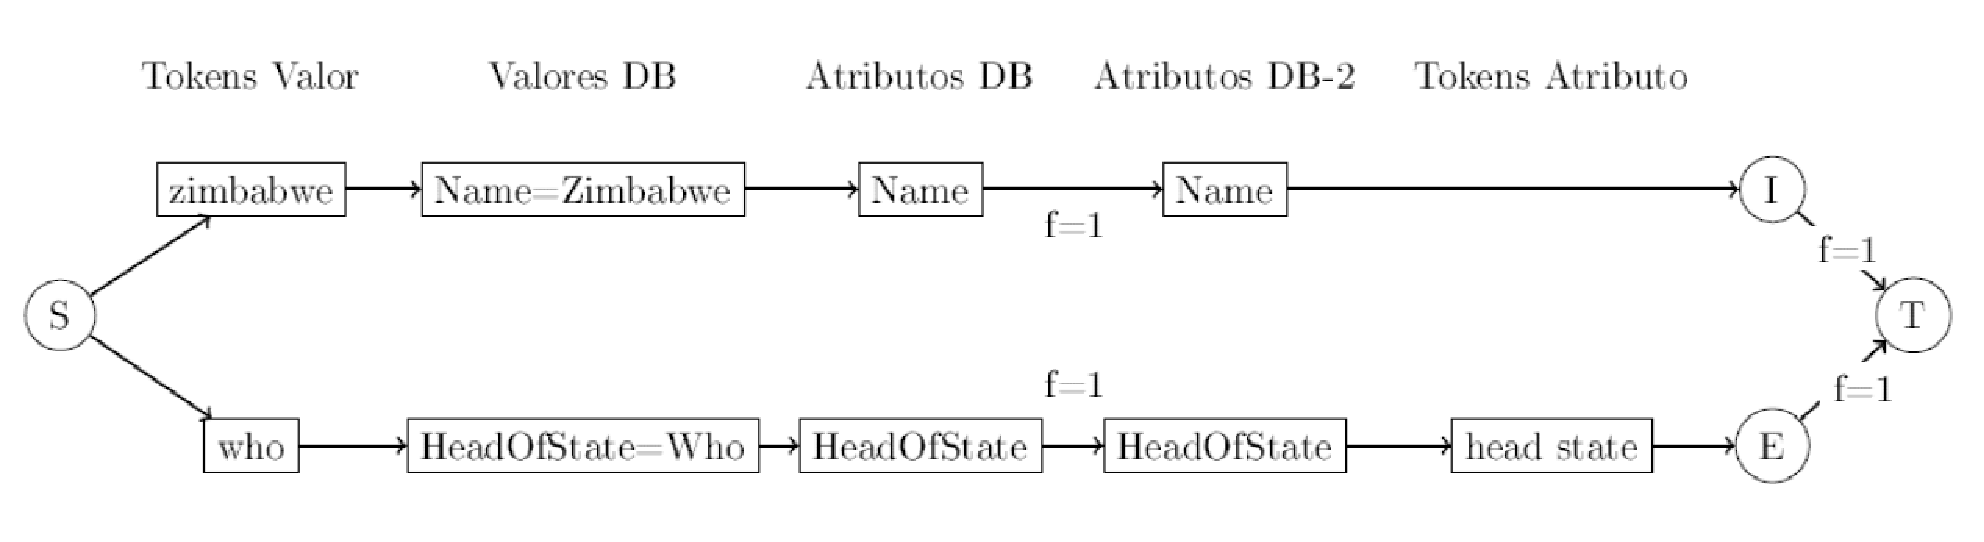
\includegraphics[scale=.33]{graficos/presentacion/ejemplo-grafo-matcher-1-6}
\end{figure}
\end{frame}
\begin{frame}[t]
\frametitle{Ejemplo 1: Matcher - notas}
\Large{``{\color{blue}Who} \st{is} \st{the} {\color{blue}head} \st{of} {\color{blue}state} \st{of} {\color{purple}Zimbabwe}?''}
\normalsize{
\begin{itemize}
  \item {\color{blue}head state} es el atributo {\color{blue}Country.HeadOfState}
  \item {\color{blue}Who} es un valor (especial) de {\color{blue}Country.HeadOfState}
  \item {\color{purple}Zimbabwe} es un valor de Country.Name ({\color{purple}implícito})
  \item No desambigua nada (los tokens tiene un solo elemento asociado)
\end{itemize}
}
\bigskip
Los tokens `who' y `head state' deben estar sintácticamente asociados

\end{frame}
\begin{frame}[t]
\frametitle{Ejemplo 1: Matcher - Asociación sintáctica - Regla 1}
\Large{Regla 1: who $\rightarrow$ head}
\begin{center}
\begin{figure}
  \centering
    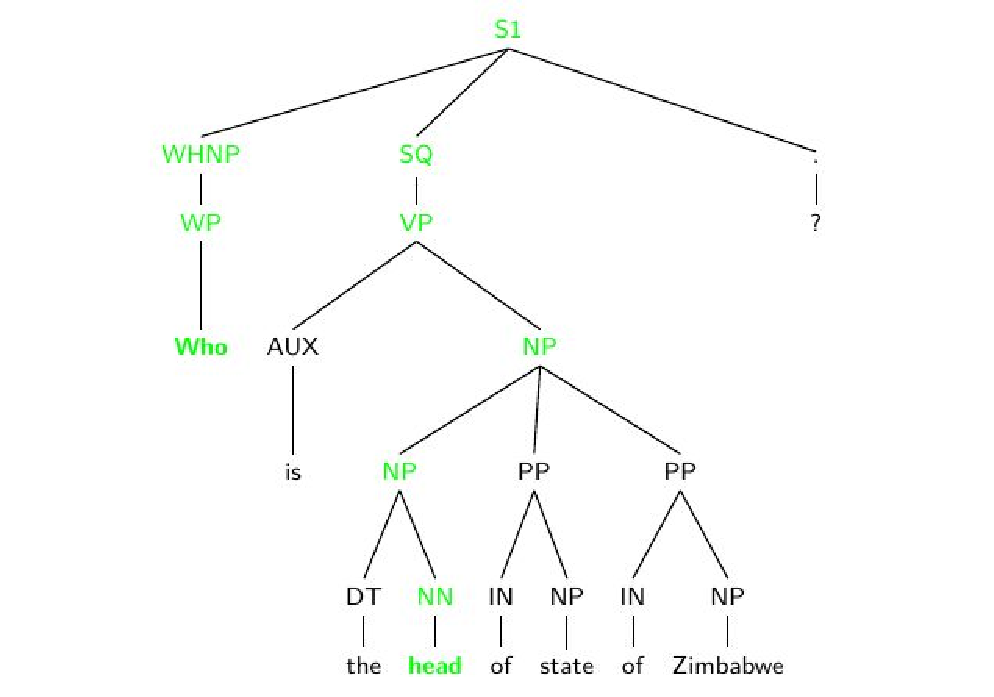
\includegraphics[scale=.5]{graficos/presentacion/ejemplo-charniak-2}
\end{figure}

\end{center}
\end{frame}

\begin{frame}[t]
\frametitle{Ejemplo 1: Matcher - Asociación sintáctica - Regla 6}
\Large{Regla 6: head $\rightarrow$ state}
\begin{center}

\begin{figure}
  \centering
    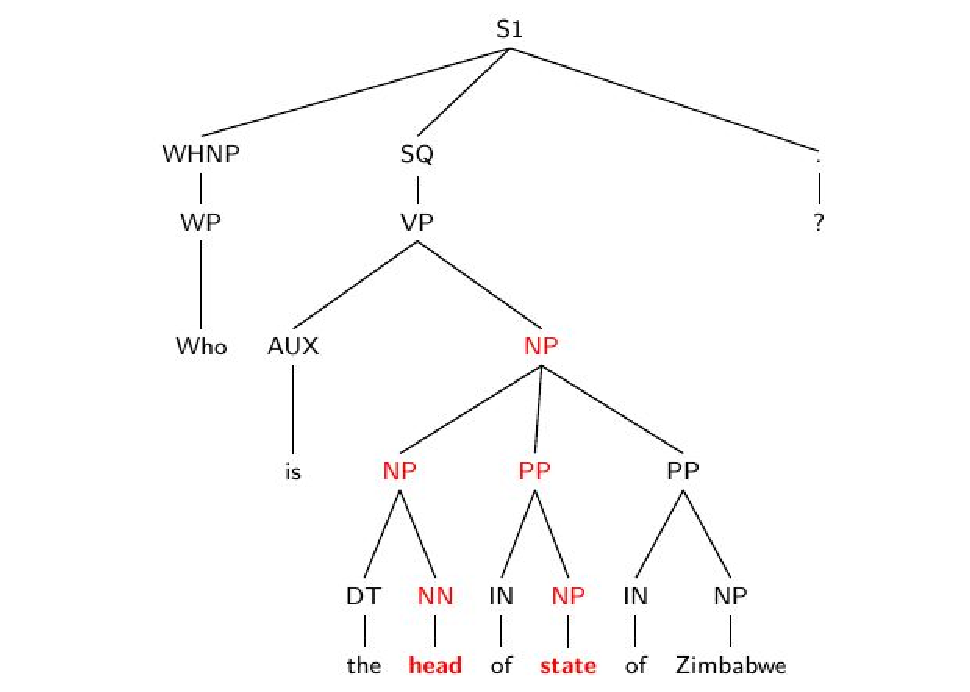
\includegraphics[scale=.5]{graficos/presentacion/ejemplo-charniak-1}
\end{figure}
\end{center}
\end{frame}

\begin{frame}[t]
\frametitle{Ejemplo 1: Generador de Queries}
\Large{Who is the head of state of Zimbabwe? 
\bigskip
\newline
{\color{white}\textbf{{\color{white}SELECT}} HeadOfState \newline
{\color{white}\textbf{FROM}} Country \newline
{\color{white}\textbf{WHERE}} Country.Name$=$ {\color{white}`Zimbabwe'}
}}

\bigskip

{\color{white}\textbf{``Robert G. Mugabe''}}

\end{frame}



\begin{frame}[t]
\frametitle{Ejemplo 1: Generador de Queries}
\Large{{\color{blue}Who} \st{is} \st{the} {\color{blue}head} \st{of} {\color{blue}state} \st{of} {\color{purple}Zimbabwe}? 
\bigskip
\newline
{\color{white}\textbf{{\color{white}SELECT}} HeadOfState \newline
{\color{white}\textbf{FROM}} Country \newline
{\color{white}\textbf{WHERE}} Country.Name$=$ {\color{white}`Zimbabwe'}
}}

\bigskip

{\color{white}\textbf{``Robert G. Mugabe''}}

\end{frame}

\begin{frame}[t]
\frametitle{Ejemplo 1: Generador de Queries}
\Large{{\color{blue}Who} \st{is} \st{the} {\color{blue}head} \st{of} {\color{blue}state} \st{of} {\color{purple}Zimbabwe}? 
\bigskip
\newline
\textbf{{\color{blue}Who}} $\rightarrow$ Valor de Country.HeadOfState \newline
\textbf{{\color{blue}head state}} $\rightarrow$ Atributo Country.HeadOfState \newline
\textbf{{\color{purple}Zimbabwe}} $\rightarrow$ Valor implícito de Country.Name \newline
}

\bigskip

{\color{white}\textbf{``Robert G. Mugabe''}}

\end{frame}

\begin{frame}[t]
\frametitle{Ejemplo 1: Generador de Queries}
\Large{{\color{blue}Who} \st{is} \st{the} {\color{blue}head} \st{of} {\color{blue}state} \st{of} {\color{purple}Zimbabwe}? 
\bigskip
\newline
\textbf{{\color{purple}SELECT}} HeadOfState \newline
{\color{purple}\textbf{FROM}} Country \newline
{\color{purple}\textbf{WHERE}} Country.Name$=$ {\color{green}`Zimbabwe'}
}

\bigskip

\textbf{``Robert G. Mugabe''}

\end{frame}



\begin{frame}
\frametitle{Ejemplo 2: What caribbean countries are also considered north american?}
  \begin{enumerate}
    \item {\color{red}FILL ME}
  \end{enumerate}
\end{frame}

\subsubsection*{Conclusiones y limitaciones}
\begin{frame}
\frametitle{Conclusiones y limitaciones}
  \begin{itemize}
    \item {\color{red} FILL ME}
  \end{itemize}
\end{frame}
